\documentclass[11pt]{article}
\usepackage[letterpaper,margin=0.85in]{geometry}
\usepackage{amsmath,amssymb}
\usepackage{tikz}
\usetikzlibrary{arrows.meta}
\usepackage{xcolor}
\usepackage{enumitem}
\usepackage{fancyhdr}
\usepackage{titlesec}
\usepackage{tabularx}
\usepackage{setspace}

\definecolor{gold}{HTML}{8A6D3B}
\definecolor{ansred}{HTML}{C0392B}

\titleformat{\section}{\centering\bfseries\large\color{gold}}{}{0pt}{}
\titlespacing{\section}{0pt}{6pt}{10pt}

\pagestyle{empty}
\setlength{\parindent}{0pt}
\setlength{\parskip}{2pt}

% ---------- helper commands ----------

% blank coordinate grid, -10 to 10
\newcommand{\blankgrid}{%
\begin{center}
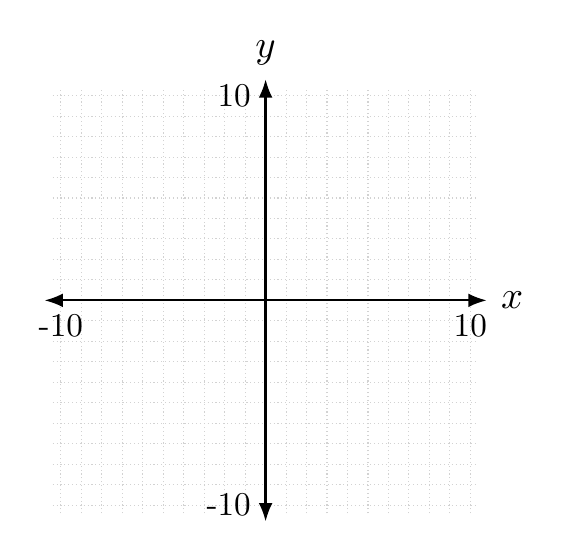
\begin{tikzpicture}[scale=0.26]
  \foreach \i in {-10,...,10}{
    \draw[gray!35,densely dotted,thin] (\i,-10.4) -- (\i,10.4);
    \draw[gray!35,densely dotted,thin] (-10.4,\i) -- (10.4,\i);
  }
  \draw[Latex-Latex,thick] (-10.8,0) -- (10.8,0) node[right,scale=1.4]{$x$};
  \draw[Latex-Latex,thick] (0,-10.8) -- (0,10.8) node[above,scale=1.4]{$y$};
  \node[below,scale=1.2] at (10,-0.15) {10};
  \node[below,scale=1.2] at (-10,-0.15) {-10};
  \node[left,scale=1.2] at (-0.15,10) {10};
  \node[left,scale=1.2] at (-0.15,-10) {-10};
\end{tikzpicture}
\end{center}}

% answer-key grid: draws the line y = m x + b across the -10..10 window
\newcommand{\answergrid}[2]{%
\begin{center}
\begin{tikzpicture}[scale=0.26]
  \foreach \i in {-10,...,10}{
    \draw[gray!35,densely dotted,thin] (\i,-10.4) -- (\i,10.4);
    \draw[gray!35,densely dotted,thin] (-10.4,\i) -- (10.4,\i);
  }
  \draw[Latex-Latex,thick] (-10.8,0) -- (10.8,0) node[right,scale=1.4]{$x$};
  \draw[Latex-Latex,thick] (0,-10.8) -- (0,10.8) node[above,scale=1.4]{$y$};
  \node[below,scale=1.2] at (10,-0.15) {10};
  \node[below,scale=1.2] at (-10,-0.15) {-10};
  \node[left,scale=1.2] at (-0.15,10) {10};
  \node[left,scale=1.2] at (-0.15,-10) {-10};
  \draw[ansred,very thick,domain=-10.6:10.6,samples=2]
    plot(\x,{(#1)*\x+(#2)});
  \fill[ansred] (0,{#2}) circle (2.6pt);
\end{tikzpicture}
\end{center}}

% blank number line, -10 to 10
\newcommand{\blanknumberline}{%
\begin{center}
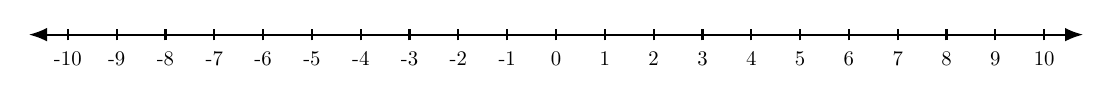
\begin{tikzpicture}[scale=0.62]
  \draw[Latex-Latex,thick] (-10.8,0) -- (10.8,0);
  \foreach \i in {-10,...,10}{
    \draw[thick] (\i,-0.12) -- (\i,0.12);
    \node[below,scale=0.75] at (\i,-0.2) {\i};
  }
\end{tikzpicture}
\end{center}}

% answer-key number line: bounds lo/hi, filled=1 for closed circle, 0 for open,
% labels drawn above the circles
\newcommand{\answernumberline}[5]{%
\begin{center}
\begin{tikzpicture}[scale=0.62]
  \draw[Latex-Latex,thick] (-10.8,0) -- (10.8,0);
  \foreach \i in {-10,...,10}{
    \draw[thick] (\i,-0.12) -- (\i,0.12);
    \node[below,scale=0.75] at (\i,-0.2) {\i};
  }
  \draw[ansred,line width=3pt] (#1,0) -- (#2,0);
  \ifnum#3=1
    \fill[ansred] (#1,0) circle (4.2pt);
    \fill[ansred] (#2,0) circle (4.2pt);
  \else
    \draw[ansred,fill=white,line width=1.4pt] (#1,0) circle (4.2pt);
    \draw[ansred,fill=white,line width=1.4pt] (#2,0) circle (4.2pt);
  \fi
  \node[above,ansred,scale=0.85] at (#1,0.28) {#4};
  \node[above,ansred,scale=0.85] at (#2,0.28) {#5};
\end{tikzpicture}
\end{center}}

\newcommand{\worklines}[1]{%
  \vspace{2pt}
  \foreach \n in {1,...,#1}{\par\vspace{18pt}\hrule height 0.4pt}
  \vspace{4pt}}

\newcommand{\field}[2]{\textbf{#1:} \makebox[#2]{\hrulefill}}

\newcommand{\worksheetheader}[1]{%
\begin{center}
  {\bfseries\Large ALGEBRA 2}\\[2pt]
  {\itshape\color{gray} Extra Practice --- Chapter 1 $\bullet$ #1}
\end{center}
\vspace{2pt}
Name: \makebox[2.6in]{\hrulefill} \hfill Date: \makebox[1.1in]{\hrulefill} \hfill Period: \makebox[0.6in]{\hrulefill}\\[2pt]
\hrule height 0.6pt
\textbf{\footnotesize SHOW ALL WORK.}\\
\hrule height 0.6pt
\vspace{4pt}}

\newcommand{\ptval}[1]{~{\footnotesize\itshape\color{gray!70!black}(#1 points)}}

% ================================================================
\begin{document}

% ---------------- PRACTICE SET 1 ----------------
\worksheetheader{Practice Set 1}

\begin{enumerate}[leftmargin=1.6em,label=\arabic*.,itemsep=10pt]
\item Solve $\dfrac{3}{4}(3x-4)-\dfrac{1}{6}(2x-5)=\dfrac{1}{2}(4x+1)$. \ptval{4}
\worklines{3}

\item Find the value of $r$ so that the line passes through $\left(\dfrac{1}{4},-\dfrac{1}{2}\right)$ and $\left(r,\dfrac{3}{4}\right)$ with the slope $\dfrac{5}{8}$. \ptval{4}
\worklines{3}
\field{$r=$}{1.4in}
\end{enumerate}

\section*{3 -- 4. \normalfont\normalsize Write an equation of the line that satisfies the given conditions and identify its rate of change.}
\vspace{-4pt}

\begin{enumerate}[leftmargin=1.6em,start=3,label=\arabic*.,itemsep=10pt]
\item Passing through $(-3,5)$ and $(1,-3)$ \ptval{5}
\worklines{3}
\field{Rate of change}{1in}

\item Passing through $(2,-1)$ and perpendicular to $2x+4y=8$ \ptval{5}
\worklines{3}
\field{Rate of change}{1in}
\end{enumerate}

\begin{enumerate}[leftmargin=1.6em,start=5,label=\arabic*.,itemsep=10pt]
\item Solve $5-3|2x-1|>-4$, graph the inequality, and write the inequality in interval notation. \ptval{6}
\worklines{3}
\field{Inequality}{2.4in}
\blanknumberline
\field{Interval notation}{2.4in}

\item Graph $y-3=\dfrac{1}{2}(x-4)$. Then find the slope and the $y$-intercept. \ptval{6}
\field{Slope}{0.9in} \hfill \field{$y$-intercept}{0.9in}
\blankgrid
\end{enumerate}

\clearpage
% ---------------- PRACTICE SET 2 ----------------
\worksheetheader{Practice Set 2}

\begin{enumerate}[leftmargin=1.6em,label=\arabic*.,itemsep=10pt]
\item Solve $\dfrac{3}{4}(3x-5)-\dfrac{1}{2}(x-3)=\dfrac{1}{2}(4x-2)$. \ptval{4}
\worklines{3}

\item Find the value of $r$ so that the line passes through $\left(\dfrac{1}{3},-\dfrac{1}{6}\right)$ and $\left(r,\dfrac{5}{6}\right)$ with the slope $\dfrac{2}{3}$. \ptval{4}
\worklines{3}
\field{$r=$}{1.4in}
\end{enumerate}

\section*{3 -- 4. \normalfont\normalsize Write an equation of the line that satisfies the given conditions and identify its rate of change.}
\vspace{-4pt}

\begin{enumerate}[leftmargin=1.6em,start=3,label=\arabic*.,itemsep=10pt]
\item Passing through $(0,-3)$ and $(4,5)$ \ptval{5}
\worklines{3}
\field{Rate of change}{1in}

\item Passing through $(-4,1)$ and perpendicular to $3x-6y=12$ \ptval{5}
\worklines{3}
\field{Rate of change}{1in}
\end{enumerate}

\begin{enumerate}[leftmargin=1.6em,start=5,label=\arabic*.,itemsep=10pt]
\item Solve $7-2|3x+1|\geq -3$, graph the inequality, and write the inequality in interval notation. \ptval{6}
\worklines{3}
\field{Inequality}{2.4in}
\blanknumberline
\field{Interval notation}{2.4in}

\item Graph $y+2=-3(x-1)$. Then find the slope and the $y$-intercept. \ptval{6}
\field{Slope}{0.9in} \hfill \field{$y$-intercept}{0.9in}
\blankgrid
\end{enumerate}

\clearpage
% ---------------- PRACTICE SET 3 ----------------
\worksheetheader{Practice Set 3}

\begin{enumerate}[leftmargin=1.6em,label=\arabic*.,itemsep=10pt]
\item Solve $\dfrac{5}{6}(3x-2)-\dfrac{1}{2}(2x-1)=\dfrac{1}{3}(6x+4)$. \ptval{4}
\worklines{3}

\item Find the value of $r$ so that the line passes through $\left(-\dfrac{1}{2},\dfrac{1}{4}\right)$ and $\left(r,-\dfrac{3}{4}\right)$ with the slope $-\dfrac{5}{6}$. \ptval{4}
\worklines{3}
\field{$r=$}{1.4in}
\end{enumerate}

\section*{3 -- 4. \normalfont\normalsize Write an equation of the line that satisfies the given conditions and identify its rate of change.}
\vspace{-4pt}

\begin{enumerate}[leftmargin=1.6em,start=3,label=\arabic*.,itemsep=10pt]
\item Passing through $(4,-1)$ and $(-4,3)$ \ptval{5}
\worklines{3}
\field{Rate of change}{1in}

\item Passing through $(2,3)$ and perpendicular to $5x+2y=10$ \ptval{5}
\worklines{3}
\field{Rate of change}{1in}
\end{enumerate}

\begin{enumerate}[leftmargin=1.6em,start=5,label=\arabic*.,itemsep=10pt]
\item Solve $6-4|2x-3|>-10$, graph the inequality, and write the inequality in interval notation. \ptval{6}
\worklines{3}
\field{Inequality}{2.4in}
\blanknumberline
\field{Interval notation}{2.4in}

\item Graph $y-1=-\dfrac{2}{3}(x+3)$. Then find the slope and the $y$-intercept. \ptval{6}
\field{Slope}{0.9in} \hfill \field{$y$-intercept}{0.9in}
\blankgrid
\end{enumerate}

\clearpage
% ================================================================
\begin{center}
{\bfseries\LARGE ANSWER KEY}\\[3pt]
{\itshape\color{gray} Algebra 2 --- Extra Practice, Chapter 1}
\end{center}
\vspace{6pt}

\section*{Practice Set 1 --- Answer Key}
\begin{enumerate}[leftmargin=1.6em,label=\arabic*.,itemsep=8pt]
\item Distribute: $2x-\frac{8}{3}-\left(\frac13 x-\frac56\right)=2x+\frac12$ $\;\to\;$ Combine: $\frac53x-\frac{11}{6}=2x+\frac12$ $\;\to\;$ $-\frac13 x=\frac12+\frac{11}{6}=\frac73$\\
\textbf{\color{ansred}Answer: $x=-7$}

\item $\dfrac58=\dfrac{\frac34-(-\frac12)}{r-\frac14}=\dfrac{5/4}{r-1/4}$ $\;\to\;$ $r-\frac14=\frac54\div\frac58=2$\\
\textbf{\color{ansred}Answer: $r=\dfrac{9}{4}$}

\item $m=\dfrac{-3-5}{1-(-3)}=\dfrac{-8}{4}=-2$ $\;\to\;$ $y-5=-2(x+3)\;\to\;y=-2x-1$\\
\textbf{\color{ansred}Answer: $y=-2x-1$;\ \ rate of change $=-2$}

\item $2x+4y=8\to y=-\frac12x+2$, given slope $=-\frac12$ $\;\to\;$ perpendicular slope $=2$; $\;y-(-1)=2(x-2)$\\
\textbf{\color{ansred}Answer: $y=2x-5$;\ \ rate of change $=2$}

\item $-3|2x-1|>-9\to|2x-1|<3\to -3<2x-1<3\to -2<2x<4$\\
\textbf{\color{ansred}Answer: $-1<x<2$;\ \ interval notation $(-1,2)$}
\answernumberline{-1}{2}{0}{-1}{2}

\item $y=\frac12x-2+3=\frac12x+1$\\
\textbf{\color{ansred}Answer: slope $=\dfrac12$;\ \ $y$-intercept $=1$}
\answergrid{0.5}{1}
\end{enumerate}

\clearpage
\section*{Practice Set 2 --- Answer Key}
\begin{enumerate}[leftmargin=1.6em,label=\arabic*.,itemsep=8pt]
\item Distribute: $\frac94x-\frac{15}{4}-\left(\frac12x-\frac32\right)=2x-1$ $\;\to\;$ Combine: $\frac74x-\frac94=2x-1$ $\;\to\;$ $-\frac14x=-1+\frac94=\frac54$\\
\textbf{\color{ansred}Answer: $x=-5$}

\item $\dfrac23=\dfrac{\frac56-(-\frac16)}{r-\frac13}=\dfrac{1}{r-1/3}$ $\;\to\;$ $r-\frac13=\frac32$\\
\textbf{\color{ansred}Answer: $r=\dfrac{11}{6}$}

\item $m=\dfrac{5-(-3)}{4-0}=\dfrac84=2$ $\;\to\;$ $y-(-3)=2(x-0)\;\to\;y=2x-3$\\
\textbf{\color{ansred}Answer: $y=2x-3$;\ \ rate of change $=2$}

\item $3x-6y=12\to y=\frac12x-2$, given slope $=\frac12$ $\;\to\;$ perpendicular slope $=-2$; $\;y-1=-2(x+4)$\\
\textbf{\color{ansred}Answer: $y=-2x-7$;\ \ rate of change $=-2$}

\item $-2|3x+1|\geq -10\to|3x+1|\leq5\to -5\leq3x+1\leq5\to -6\leq3x\leq4$\\
\textbf{\color{ansred}Answer: $-2\leq x\leq\dfrac43$;\ \ interval notation $\left[-2,\dfrac43\right]$}
\answernumberline{-2}{1.333}{1}{-2}{4/3}

\item $y=-3x+3-2=-3x+1$\\
\textbf{\color{ansred}Answer: slope $=-3$;\ \ $y$-intercept $=1$}
\answergrid{-3}{1}
\end{enumerate}

\clearpage
\section*{Practice Set 3 --- Answer Key}
\begin{enumerate}[leftmargin=1.6em,label=\arabic*.,itemsep=8pt]
\item Distribute: $\frac52x-\frac53-\left(x-\frac12\right)=2x+\frac43$ $\;\to\;$ Combine: $\frac32x-\frac76=2x+\frac43$ $\;\to\;$ $-\frac12x=\frac43+\frac76=\frac52$\\
\textbf{\color{ansred}Answer: $x=-5$}

\item $-\dfrac56=\dfrac{-\frac34-\frac14}{r-(-\frac12)}=\dfrac{-1}{r+1/2}$ $\;\to\;$ $r+\frac12=-1\div\left(-\frac56\right)=\frac65$\\
\textbf{\color{ansred}Answer: $r=\dfrac{7}{10}$}

\item $m=\dfrac{3-(-1)}{-4-4}=\dfrac{4}{-8}=-\dfrac12$ $\;\to\;$ $y-(-1)=-\frac12(x-4)\;\to\;y=-\frac12x+1$\\
\textbf{\color{ansred}Answer: $y=-\dfrac12x+1$;\ \ rate of change $=-\dfrac12$}

\item $5x+2y=10\to y=-\frac52x+5$, given slope $=-\frac52$ $\;\to\;$ perpendicular slope $=\frac25$; $\;y-3=\frac25(x-2)$\\
\textbf{\color{ansred}Answer: $y=\dfrac25x+\dfrac{11}{5}$;\ \ rate of change $=\dfrac25$}

\item $-4|2x-3|>-16\to|2x-3|<4\to -4<2x-3<4\to -1<2x<7$\\
\textbf{\color{ansred}Answer: $-\dfrac12<x<\dfrac72$;\ \ interval notation $\left(-\dfrac12,\dfrac72\right)$}
\answernumberline{-0.5}{3.5}{0}{-1/2}{7/2}

\item $y=-\frac23x-2+1=-\frac23x-1$\\
\textbf{\color{ansred}Answer: slope $=-\dfrac23$;\ \ $y$-intercept $=-1$}
\answergrid{-0.667}{-1}
\end{enumerate}

\end{document}
